\documentclass{beamer}
\usepackage[utf8]{inputenc}

\usetheme{Madrid}
\usecolortheme{default}
\usepackage{amsmath,amssymb,amsfonts,amsthm}
\usepackage{txfonts}
\usepackage{tkz-euclide}
\usepackage{listings}
\usepackage{adjustbox}
\usepackage{array}
\usepackage{tabularx}
\usepackage{gvv}
\usepackage{lmodern}
\usepackage{circuitikz}
\usepackage{tikz}
\usepackage[utf8]{inputenc}
\usepackage{extarrows}
\usetheme{Madrid}
\usecolortheme{default}
\usepackage{amsmath,amssymb,amsfonts,amsthm}
\usepackage{txfonts}
\usepackage{tkz-euclide}
\usepackage{listings}
\usepackage{adjustbox}
\usepackage{array}
\usepackage{tabularx}
\usepackage{gvv}
\usepackage{lmodern}
\usepackage{circuitikz}
\usepackage{tikz}
\usepackage{graphicx}
\usepackage{amsmath} 

\setbeamertemplate{page number in head/foot}[totalframenumber]

\usepackage{tcolorbox}
\tcbuselibrary{minted,breakable,xparse,skins}



\definecolor{bg}{gray}{0.95}
\DeclareTCBListing{mintedbox}{O{}m!O{}}{%
  breakable=true,
  listing engine=minted,
  listing only,
  minted language=#2,
  minted style=default,
  minted options={%
    linenos,
    gobble=0,
    breaklines=true,
    breakafter=,,
    fontsize=\small,
    numbersep=8pt,
    #1},
  boxsep=0pt,
  left skip=0pt,
  right skip=0pt,
  left=25pt,
  right=0pt,
  top=3pt,
  bottom=3pt,
  arc=5pt,
  leftrule=0pt,
  rightrule=0pt,
  bottomrule=2pt,

  colback=bg,
  colframe=orange!70,
  enhanced,
  overlay={%
    \begin{tcbclipinterior}
    \fill[orange!20!white] (frame.south west) rectangle ([xshift=20pt]frame.north west);
    \end{tcbclipinterior}},
  #3,
}
\lstset{
    language=C,
    basicstyle=\ttfamily\small,
    keywordstyle=\color{blue},
    stringstyle=\color{orange},
    commentstyle=\color{green!60!black},
    numbers=left,
    numberstyle=\tiny\color{gray},
    breaklines=true,
    showstringspaces=false,
}
\title %optional
{4.13.37}

\author 
{Kartik Lahoti - EE25BTECH11032}

\begin{document}


\frame{\titlepage}
\begin{frame}{Question}
If $x_1 , x_2 , x_3$ as well as $y_1 , y_2 ,y _3$, are in G.P with the same common ratio then then points $\brak{x_1 , y_1}$, $\brak{x_2 , y_2}$ and $\brak{x_3 , y_3}$
\begin{multicols}
\begin{enumerate}
        \item lie on a straight line
        \item lie on ellipse 
        \item lie on circle
        \item are vertices of a triangle
    
\end{enumerate}
\end{multicols}
\end{frame}

\begin{frame}{Theoretical Solution}
    \begin{table}[]
        \centering
        \begin{tabular}{|c|c|}
\hline
\textbf{Name} & \textbf{Value} \\ \hline
$\vec{A}$ & $\myvec{2 & 1 \\0 & 3}$ \\ \hline
\end{tabular}

        \caption{$4.13.37$}
        \label{tab:1.0}
    \end{table}
\end{frame}

\begin{frame}{Theoretical Solution}

To check if $\vec{A}$ , $\vec{B}$ and $\vec{C}$ lie on a straight line , 

\begin{align}
    rank\myvec{\vec{B} - \vec{A} & \vec{C} - \vec{B}} = 1
\end{align}

If $r$ is the common ratio for the G.P , then vector $\vec{B}$ and $\vec{C}$ can also be written as

\begin{align}
    \vec{B} = r\vec{A} \hspace{1cm} \vec{C} = r^2\vec{A} 
\end{align}

\end{frame}
\begin{frame}{Theoretical Solution}

\begin{align}
    rank\myvec{r\vec{A} - \vec{A} & r^2\vec{A} - r\vec{A} } = 1 
\end{align}

Case $1\colon$ $x_1 \neq 0 $ 

\begin{align}
    \brak{r-1}\myvec{x_1 & rx_1 \\ y_1 & ry_1} \xleftrightarrow[]{R_2 \rightarrow {R_2 - \frac{y_1}{x_1}R_1 }} \myvec{x_1 & rx_1 \\ 0 & 0 }
\end{align}

\end{frame}
\begin{frame}{Theoretical Solution}

Case $2\colon$ $\brak{x_1 = 0  \text{ and }  y_1 \neq 0}$ or $\brak{x_1 \neq 0 \text{ and }  y_1 = 0 }$

\begin{align}
    \myvec{0 & 0 \\ y_1 & ry_1} \hspace{0.5cm}or\hspace{0.5cm} \myvec{x_1 & rx_1 \\ 0 & 0} 
\end{align}

From Case $1$ and Case $2$ we can see $rank = 1$. Thus, the points lie on a straight line

Hence, Answer $\colon \brak{1}$
\end{frame}



\begin{frame}[fragile]
    \frametitle{C Code (1)}

    \begin{lstlisting}
void gp( double *X , double *Y , double fact  )
{
	for(int i= 0 ; i <2 ; i++)
			Y[i] = X[i] * fact;
}

\end{lstlisting}
\end{frame}

\begin{frame}[fragile]
    \frametitle{C Code (2) - Function to Generate Points on Line}
    \begin{lstlisting}
    
void linegen(double *XY, double *A , double *B , int n , int m )
{
    double temp[m] ; 
    for (int i = 0 ; i < m ; i++)
    {
        temp [ i ] = (B[i]- A[i]) /(double) n ; 
    }
    for (int i = 0 ; i < n ; i++ )
        for (int j = 0 ; j < m ; j++)
            XY[j*n + i ] = A[j] + temp[j] * i ; 
           
}

\end{lstlisting}
\end{frame}

\begin{frame}[fragile]
    \frametitle{Python Code - Using Shared Object}
    \begin{lstlisting}
import ctypes as ct
import numpy as np
import matplotlib.pyplot as plt

handc1 = ct.CDLL("./func.so")

handc1.gp.argtypes = [
    ct.POINTER(ct.c_double),
    ct.POINTER(ct.c_double),
    ct.c_double
]

handc1.gp.restype = None

\end{lstlisting}
\end{frame}

\begin{frame}[fragile]
    \frametitle{Python Code - Using Shared Object}
    \begin{lstlisting}

O = np.zeros(2 , dtype = np.float64).reshape(-1,1)
A = np.array([1,2] , dtype = np.float64).reshape(-1,1)
B = np.zeros(2 , dtype = np.float64).reshape(-1,1)
C = np.zeros(2, dtype = np.float64).reshape(-1,1)
r = 3 
handc1.gp(
    A.ctypes.data_as(ct.POINTER(ct.c_double)),
    B.ctypes.data_as(ct.POINTER(ct.c_double)),
    r)
handc1.gp(
    A.ctypes.data_as(ct.POINTER(ct.c_double)),
    C.ctypes.data_as(ct.POINTER(ct.c_double)),
    r**2)
print("Vector A = ",A)
print("Vector B = " , B)
print("Vector C = " , C)

\end{lstlisting}
\end{frame}

\begin{frame}[fragile]
    \frametitle{Python Code - Using Shared Object}
    \begin{lstlisting}

def line(P: np.ndarray , Q: np.ndarray, str1 , str2):
    handc2 = ct.CDLL("./line_gen.so")

    handc2.linegen.argtypes = [
        ct.POINTER(ct.c_double),
        ct.POINTER(ct.c_double),
        ct.POINTER(ct.c_double),
        ct.c_int , ct.c_int
    ]
    handc2.linegen.restype = None
    
\end{lstlisting}
\end{frame}
\begin{frame}[fragile]
    \frametitle{Python Code - Using Shared Object}
    \begin{lstlisting}
    n = 200
    XY = np.zeros((2,n),dtype=np.float64)

    handc2.linegen (
        XY.ctypes.data_as(ct.POINTER(ct.c_double)),
        P.ctypes.data_as(ct.POINTER(ct.c_double)),
        Q.ctypes.data_as(ct.POINTER(ct.c_double)),
        n,2
    )
    plt.plot(XY[0,:],XY[1,:], str1 , label = str2 )
    \end{lstlisting}
\end{frame}

\begin{frame}[fragile]
    \frametitle{Python Code - Using Shared Object}
    \begin{lstlisting}
    
plt.figure()

line(O,A,"g-"," Line Segment : OA ")
line(A,B,"r-"," Line Segment : AB ")
line(B,C,"b-"," Line Segment : BC ")

coords = np.block([[A,B,C,O]])

plt.scatter(coords[0,:] , coords[1,:])
vert_label = ['A','B','C','O']

\end{lstlisting}
\end{frame}
\begin{frame}[fragile]
    \frametitle{Python Code - Using Shared Object}
    \begin{lstlisting}
for i , txt in enumerate(vert_label) :
    
    if i != 2 :
        plt.annotate(f"{txt}\n({coords[0,i]:.1f},{coords[1,i]:.1f})",
                    (coords[0,i], coords[1,i]),
                    textcoords = "offset points" ,
                    xytext = (0,12),ha = "center")
    else :
        plt.annotate(f"{txt}\n({coords[0,i]:.1f},{coords[1,i]:.1f})",
                    (coords[0,i], coords[1,i]),
                    textcoords = "offset points" ,
                    xytext = (0,-25),ha = "center")
\end{lstlisting}
\end{frame}
\begin{frame}[fragile]
    \frametitle{Python Code - Using Shared Object}
    \begin{lstlisting}
    
plt.xlabel("$x$")
plt.ylabel("$y$")
plt.grid()

plt.legend(loc="best")

plt.title("4.13.37")

plt.savefig("../figs/colli1.png")
plt.show()

#plt.savefig('../figs/colli1.png')
#subprocess.run(shlex.split("termux-open ../figs/colli1.png"))

\end{lstlisting}
\end{frame}

\begin{frame}[fragile]
    \frametitle{Python Code}
    \begin{lstlisting}
mport math
import sys 
sys.path.insert(0, '/home/kartik-lahoti/matgeo/codes/CoordGeo')
import numpy as np
import numpy.linalg as LA
import matplotlib.pyplot as plt

from line.funcs import *

#if using termux
#import subprocess
#import shlex
\end{lstlisting}
\end{frame}

\begin{frame}[fragile]
    \frametitle{Python Code }
    \begin{lstlisting}
O = np.zeros(2).reshape(-1,1)
A = np.array([1,2]).reshape(-1,1)
B = np.zeros(2).reshape(-1,1)
C = np.zeros(2).reshape(-1,1)
r = 3 
B = r * A
C = (r ** 2 ) *A

print("Vector A = " , A)
print("Vector B = " , B)
print("Vector C = " , C)

\end{lstlisting}
\end{frame}

\begin{frame}[fragile]
    \frametitle{Python Code }
    \begin{lstlisting}
def plot_it(P,Q,str1,str2):
    x_l = line_gen_num(P,Q,20)
    plt.plot(x_l[0,:],x_l[1,:] , str1 , label =  str2)

plt.figure()
plot_it(O,A,"g-"," Line Segment : OA ")
plot_it(A,B,"r-"," Line Segment : AB ")
plot_it(B,C,"b-"," Line Segment : BC ")

coords = np.block([[A,B,C,O]])

plt.scatter(coords[0,:] , coords[1,:])
vert_label = ['A','B','C','O']


\end{lstlisting}
\end{frame}

\begin{frame}[fragile]
    \frametitle{Python Code }
    \begin{lstlisting}
for i , txt in enumerate(vert_label) :
    
    if i != 2 :
        plt.annotate(f"{txt}\n({coords[0,i]:.1f},{coords[1,i]:.1f})",
                    (coords[0,i], coords[1,i]),
                    textcoords = "offset points" ,
                    xytext = (0,12),ha = "center")
    else :
        plt.annotate(f"{txt}\n({coords[0,i]:.1f},{coords[1,i]:.1f})",
                    (coords[0,i], coords[1,i]),
                    textcoords = "offset points" ,
                    xytext = (0,-25),ha = "center")
                 
    \end{lstlisting}
\end{frame}
\begin{frame}[fragile]
    \frametitle{Python Code }
    \begin{lstlisting}
   
plt.xlabel('$x$')
plt.ylabel('$y$')
plt.grid()
plt.legend(loc = "best")
plt.title("Fig:4.13.37")
plt.savefig("../figs/colli2.png")
plt.show()

#plt.savefig('../figs/colli2.png')
#subprocess.run(shlex.split("termux-open ../figs/colli2.png"))

    \end{lstlisting}
\end{frame}


\begin{frame}{Plot}

Taking an example as $\vec{A} = \myvec{1 \\ 2}$ and $r=3$ , we get the following graph.

    \centering
    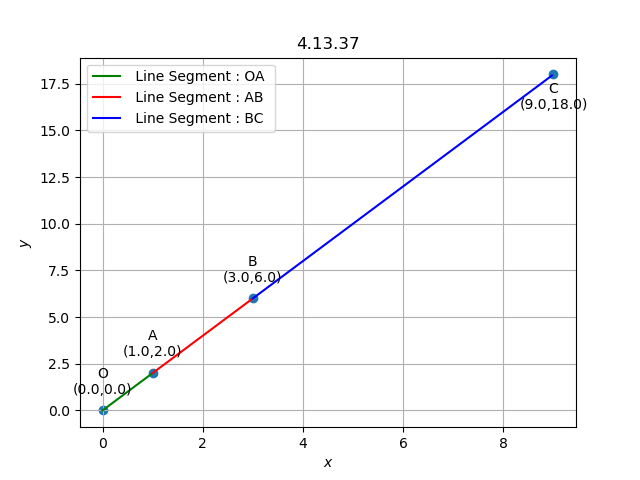
\includegraphics[width=\columnwidth, height=0.7\textheight, keepaspectratio]{../figs/colli1.png}   
\end{frame}

\end{document}
